\documentclass[12pt]{article}
\usepackage{amsmath}
\usepackage{amsthm}
\usepackage{amsfonts}
\usepackage{graphicx}
\usepackage{epstopdf}
\usepackage{float}
\usepackage{fancyhdr}
\usepackage{hyperref}
\usepackage{subcaption}
\usepackage{pdfpages}
\usepackage{algpseudocode}
\usepackage{framed}
\usepackage{amssymb}
\theoremstyle{definition}

\graphicspath{ {./eps/} } 

\makeatletter
\renewcommand\@biblabel[1]{}
\renewenvironment{thebibliography}[1]
     {\section*{\refname}%
      \@mkboth{\MakeUppercase\refname}{\MakeUppercase\refname}%
      \list{}%
           {\leftmargin0pt
            \@openbib@code
            \usecounter{enumiv}}%
      \sloppy
      \clubpenalty4000
      \@clubpenalty \clubpenalty
      \widowpenalty4000%
      \sfcode`\.\@m}
     {\def\@noitemerr
       {\@latex@warning{Empty `thebibliography' environment}}%
      \endlist}
\makeatother


\newtheorem{riskmeasure}{Definition}
\newtheorem{theorem}{Theorem}
\newtheorem{lemma}{Lemma}
\allowdisplaybreaks
%\setmainfont{Calibri}
%\pagestyle{fancy}
\fancyhf{}

\DeclareMathOperator*{\Max}{Max}
\DeclareMathOperator*{\Min}{Min}
\setlength{\parindent}{0cm}



\begin{document}

\title{Correlated latent variables in m dimensions}
\date{}
\author{Daniel H. Stahl}
\maketitle

\newpage
 
\section{Model Description}
The model setup is similar to the setup in Stahl (2015).  The main features of this model are independent defaults conditional on latent factors, mutually independent losses given default, and a semi-endogenous risk of a liquidity event.  The model in this paper distinguishes itself from Stahl (2015) in three important points.  First, the process that drives correlation is now an \(m\) dimensional process.  These processes represent the exposure of the assets to various factors.  For instance, a loan to a business in rural New Mexico or the south east may have more risk than a loan to a business in Austin or San Francisco.  A loan to a tech firm in Texas may have different risks than a loan to an energy business in Texas.  Each of these risks (geographic, industry, or otherwise) can be captured by a distinct dimension of the process.  
\\
\\
The second key difference is that these process are jointly normally distributed: in particular, by a multi-dimensional Ornstein-Uhlenbeck process.  This assumption is important for several reasons.  Normally distributed processes lend themselves to analytic tractability including the ability to easily implement a correlation structure across the factors.  The normality also allows for relatively simple transition from a CAPM and Merton type framework.  While there are many benefits to using Gaussian processes, such processes have the unfortunate property of having the positive probability of negative values.  As the probabilities of default are affine functions of the processes, this feature of Gaussian models allows for negative probabilities of default.  However, the probability of negative values need not be large; and since the integral of the process is used for determining the factors affecting the default probability the probability of having negative probabilities becomes essentially negligible.  
\\
\\
The third difference is that the risk of a liquidity crisis is an affine function of the assets' exposures.  Modeling liquidity exposure in this manner allows liquidity risk to be charged at the loan level and provides a relatively simple method to quantify and aggregate liquidity risk in terms of common funding practices like FHLB and FRB pledging.  However, this flexible modeling comes at the price of losing the linearity of the portfolio in the sense of Tasche (2007).  The main drawback is that Euler contributions no longer are the ``correct'' method for aggregating risk as the sum of the risk contributions no longer equal the entire portfolio risk.  While concerning, this drawback is overcome by using some sensible and straightforward criteria in section \ref{appXTLambda}.

This paper introduces the model and then uses examples to demonstrate how such a model may be used in an actual loan portfolio.  
\section{General framework}
In Stahl (2015), the goal was to find an analytical expression for the characteristic function of the portfolio loss so that numerical inversion could be efficiently applied to recover the density function of the loss distribution.  This paper adopts a nearly identical framework: a portfolio \(X_t=\sum_j X_t ^ j\) contains \(n\) assets \(X_t ^ j\) with mutually independent exposures \(l_j\).  Each asset has a probability of default.  In Stahl (2015) the probability of default (and correlation between defaults) was driven by a single Brownian motion; in this paper this is extended so that the instantaneous probability of default for asset \(j\) is an affine function of an \(m\) dimensional mean-reverting Levy process \(L_t\) with long run expected value equal to a vector of ones.  Letting the filtration generated by the Levy process be denoted \(\mathcal{F}_t\) and the filtration of the entire process \(X_t\) be denoted \(\mathcal{G}_t\), the probability of default for asset \(X_t ^ j\) conditioned on \(\mathcal{F}_t\) over the interval \([t, T]\) is \(\left(w_j ^ T \int_t ^ T L_s ds  \right) p_j\) where \(w_j\) is a constant normal vector, \(p_j\) is a constant, and a superscript \(T\) denotes the transpose.  Since the instantaneous default probability is \(w_j ^T L_t p_j dt\) which has long run expected value \(p_j dt\),  it is convenient to think of \(p_j\) as the long run instantaneous probability per unit time.  Following the logic in (Stahl 2015), the approximate characteristic function of \(X_T-X_t\) conditioned on \(\mathcal{G}_t\) is 
\begin{equation}
\phi_{X_T}(u)=\mathbb{E}\left[e^{\sum_j \left(w_j ^T \int_t ^ T L_s  ds \right) p_j (\phi_j(u)-1)} |\mathcal{G}_t\right]
\end{equation}
Where \(\phi_j(u)\) is the characteristic function of \(l_j\).  \(\phi_{X_T}(u)\) can be written as 

\begin{equation}
\phi_{X_T}(u)=\mathbb{E}\left[e^{\sum_k  \int_t ^ T L_s  ds \sum_j w_{j, k}  p_j (\phi_j(u)-1)} |\mathcal{G}_t\right]
\end{equation}
\begin{equation} \label{CharFY}
=\mathbb{E}\left[e^{z^T \int_t ^ T L_s  ds } |\mathcal{G}_t\right]=\mathbb{E}\left[e^{z^T (Y_T-Y_t) } |\mathcal{G}_t\right]
\end{equation}
Where \(z=\sum_j w_{j, k}  p_j (\phi_j(u)-1),\,\,k \in [1,...,m]\) and \(Y_t=\int_0 ^t L_s ds\).  But this is just the moment generating function of \(Y_t\).  As long as the moment generating function of \(Y_t\) has an analytical expression, the characteristic function has a closed form solution and can be efficiently inverted.  Examples of \(Y_t\) that satisfy this constraint in a diffusion setting can be found in Duffie et. al. (2000) while examples of \(Y_t\) that are the more general Levy process is found in  Filipovic (2001).  As far as the author knows, there is no more general formulation of the basic loss distribution.  Within the framework the problem reduces to finding suitable processes \(Y_t\).  

\section{Alternate Interpretation}

Another way to interpret the model is as follows.  Let each asset be represented by the following Levy process:
\begin{equation}
\hat{X}_T ^ j=\hat{X}_0 ^ j+\alpha_j T +\sigma_j W_T+\sum_{q=0} ^ {N_T ^ j} l_j \end{equation}
Where \(N_T\) is the counting process with parameter \(\sum_k p_j w_{j, k} Y_T ^ k\).  The characteristic function of such a process is given by

\begin{equation}
\phi(u)=\mathbb{E}\left[e^{ui \alpha_j T-\frac{u^2 \sigma_j ^2}{2} T+\left( \sum_k p_j w_{j, k} Y_T ^ k \right) (\phi_j (u)-1)} \right]
\end{equation}
This is the same characteristic function as equation (\ref{CharFY}) with the addition of a drifted Brownian motion.  With the addition of the drifted Brownian motion, it starts making more sense to consider \emph{gains} instead of \emph{losses}, so that the characteristic function reads
\begin{equation}
\hat{\phi}(u)=\mathbb{E}\left[e^{ui \alpha_j T-\frac{u^2 \sigma_j ^2}{2} T+\left( \sum_k p_j w_{j, k} Y_T ^ k \right) (\phi_j (-u)-1)} \right]
\end{equation}
Now let \(T\) itself be random: in particular, \(T=Y_T ^ 1\).  Following Carr et. al (2004), a stochastic time can be interpreted as ``business time'' instead of ``calendar time''.  A business time that moves faster than calendar time is typical of a crisis or recessionary period, and so \(T\) can be interpreted as the systemic risk in the economy.  It is natural for  \(T\) to have a long run expected value of calendar time \(t\) which, conveniently, is the long run expected value of \(Y_T ^1\).  The characteristic function then reads

\begin{equation}
\hat{\phi}(u)=\mathbb{E}\left[e^{\left(ui \alpha_j -\frac{u^2 \sigma_j ^2}{2} +p_j w_{j, 1}\left( \phi_j(-u)-1)\right) \right) Y_T ^ 1 +\left( \sum_{k>1} p_j w_{j, k} Y_T ^ k \right) (\phi_j (-u)-1)} \right]
\end{equation}

This can still be efficiently computed and inverted, with the added benefit that variations in the returns of \(X_T ^ j\) is correlated with the potential for default.  

\section{Latent Process}
For this paper, the process \(L_t\) is assumed to solve the following stochastic differential equation (SDE):

\[dL_t={A} (\mathbf{1}-{L_t}) dt +{\Sigma}d {W_t}\] 
 \({A}\) is an \(m x m\) diagonal matrix with \({A}_{i, i}>0, \,\, i = 1, ..., m\), \(\mathbf{1}\) is an \(m x 1\) vector of ones, \({\Sigma}\) is an \(m x m\) matrix satisfying \({\Sigma}{\Sigma}^T={\Omega}\) where \({\Omega}\) is positive semi-definite, and \(d{W_t}\) are independent increments of an \(m x 1\) Brownian motion.  \({\Omega}_{i, j}=\sigma_i \sigma_j \rho_{i, j},\,\,  i,\,j = 1, ...,m\) where \(\sigma_i>0\), \(\rho_{i, j} \in [-1, 1]\), and \(\rho_{i, i}=1\).

\subsection{Solution to the SDE}

By Ito's Lemma, 
\begin{equation} d\left(e^{{A}t}{L_t}\right)={A}e^{{A}t}{L_t}dt+e^{{A}t}{A} (\mathbf{1}-{L_t}) dt +e^{{A}t}{\Sigma}d {W_t} \end{equation}
The matrix exponential is, as usual, defined as \(e^{{A}}=\sum_{j=0} ^ \infty \frac{{A}^j }{j!}\).  Since \({A}\) is diagonal, this simplifies to \(\text{diag}\left(e^{A_{ii}}\right)\).
\begin{equation} d\left(e^{{A}t}{L_t}\right)=e^{{A}t}{A} \mathbf{1} dt +e^{{A}t}{\Sigma}d {W_t} \end{equation}
Integrating,
\begin{equation} e^{{A}T}{L_T}=L_0+e^{AT} \mathbf{1}-\mathbf{1}+\int_0 ^ T e^{{A}t} {\Sigma}d {W_t} \end{equation}
Solving for \(L_T\),
\begin{equation} \label{solutionL} {L_T}=e^{-AT}(L_0-\mathbf{1})+ \mathbf{1}+e^{-AT}\int_0 ^ T e^{{A}t} {\Sigma}d {W_t} \end{equation}
%\begin{equation}L_T=e^{-AT}L_0+\left[\begin{array}{c}1- e^{-{A}_{1, 1}T}\\ \vdots \\1-e^{-{A}_{m, m}T} \end{array} \right]+e^{-AT}\int_0 ^ T e^{{A}t} {\Sigma}d {W_t} %\end{equation}
As this equation is deterministic in volatility, the distribution of \(L_t\) is normal.  

\subsection{Moments of \(Y_T\)} 

Recall that the probability of default is an affine function of \(Y_T=\int_0^T L_t dt\).  Since \(L_t\) is Gaussian, the integral of \(L_t\) is also Gaussian.  The moment generating function of a Gaussian random variable with mean \(\mu\) and variance \(\sigma^2\) is the following (reference any statistics text book):

\begin{equation}\phi_{\mathrm{Gaussian}}(u)=\label{GaussianMGF} e^{u\mu +\frac{u^2\sigma^2}{2}} \end{equation}

Thus equation (\ref{CharFY}) reduces to the computation of the expectation and variance of \(z^T Y_T\).  The expectation and variance is the following:
\begin{equation} \label{meY} \mathbb{E}[z^T Y_T]=\mu(z)=\sum_{i=1} ^ m z_i T+\frac{z_i}{A_{i,i}}\left(1-e^{-{A}_{i, i}T}\right)(L_0^ i-1)\end{equation}

\begin{multline}\label{varianceY} \mathbb{V}(z^T Y_T)=\sigma^2(z)=\\ \sum_i \sum_j \rho_{i,j} \frac{ z_i z_j \sigma_i \sigma_j}{A_{i,i} A_{j,j}} \left(T-\frac{1-e^{-A_{i,i}T}}{A_{i,i}}-\frac{1-e^{-A_{j,j}T}}{A_{j,j}}+\frac{1-e^{-(A_{i,i}+A_{j,j})T}}{A_{i,i}+A_{j,j}}\right) \end{multline}

See Appendix (\ref{mY}) for a full derivation.
\section{Numerical Solution for Risk Measures}

Stahl (2015) derived a method for finding the density of the loss distribution.  Finding risk measures such as Value at Risk or Expected Shortfall required integrating this distribution numerically.  This additional integration added (small) computational overhead and additional numerical approximations.  In this paper I demonstrate how to find these measures more efficiently and with the same numerical error as finding the density itself. 
\\
\\
Following Fang and Oosterlee (2008), the domain of \(X\) is truncated between \((a,\,b)\).  The expectation 
\(\mathbb{E}[g(X)]=\int_\mathbb{R} g(x) f(x)dx \) can be approximated (for a given \(x\)) by 
\[\sum_{k=0} ^ {n-1}\delta(k)\mathrm{Re}  \left(\phi\left(\frac{\pi k}{b-a}\right) e^{-ik\pi \frac{a}{b-a}} \right) \frac{2V_k}{b-a} \]
Where \(\delta(j)=\frac{1}{2}\) if \(j=0\) and one otherwise, \(\phi(u)\) is the characteristic function of \(X\), and \[V_k=\int_{a}^{x} g(y) \cos \left(k\pi \frac{y-a}{b-a} \right) dy\] 
\subsection{Cumulative Density}

To find the CDF of \(X\), \(g(X)=1\).  Integrating to find \(V_k\) produces the following result:

\[V_k ^ {CDF}=\sin\left(k\pi \frac{x-a}{b-a}\right)\frac{b-a}{k\pi}\]
When \(k=0\) the integral is trivial to evaluate and becomes \(x-a\).   To find the Value at Risk requires solving the equation \(q(x)=\alpha\) where \(\alpha\) is the confidence level of the Value at Risk and \(q\) is the CDF.  For example, a bisection method can be used to numerically solve the equation.

\subsection{Expectation}

To find the (partial) expectation of \(X\), \(g(X)=X\).  Again integrating \(V_k\),
\[V_k ^{E}=x\sin \left(k\pi \frac{x-a}{b-a}\right)\frac{b-a}{k\pi}+\left(\frac{b-a}{k\pi}\right)^2 \left(\cos\left(k\pi \frac{x-a}{b-a}\right)-1\right)\]
When \(k=0\) this becomes \(\frac{x^2-a^2}{2}\).  The entire expectation can be found in a single summation by specifying \(x=b\).  For the purposes of computing expected shortfall, the following representation becomes convenient:
\[\rho_{ES}(X)=\frac{1}{\alpha}\mathbb{E}[-X \mathbb{I}_{X<-\rho_{VaR}}]\]

The expected shortfall can thus be found in a single summation after finding the Value at Risk as shown above by setting \(x=\rho_{VaR}\).

\section{Liquidity Risk} \label{riskContributions}
In Stahl (2015) liquidity risk is modeled by a constant exposure (fixing time) and a probability of a ``crisis'' that is linear in the dollar credit loss.  This allowed the characteristic function of the portfolio loss to retain the same analytical form.  In this paper this concept is generalized further so that the exposure in the case of a liquidity ``crisis'' is an affine function of the individual asset balances at time \(t\).  Using this method retains the analytical characteristic function but also allows liquidity capital to be pushed down to individual loans.  In the case of a liquidity event (which increases in probability as credit losses mount), loans typically must be liquidated at large discounts to par to meet obligations.  The probability of this event occurring (at time \(T\)) is \(q X_T\) where \(X_T\) is the realization of the losses within the portfolio.  In Stahl (2015) the exposure was a fixed constant \(\lambda\).  

\subsection{Characteristic function and Loss distribution Moments}
From Stahl (2015), equation (\ref{CharFY}), and equation (\ref{GaussianMGF}), the characteristic function including liquidity risk is

\begin{equation} \label{finalCH}
\phi_{X_T ^ \lambda}=e^{\mu(z^\lambda)+\frac{\sigma^2(z^\lambda)}{2} }
\end{equation}
Where \(z^\lambda=\sum_j w_{j, k}  p_j (\phi_j(u^\lambda )-1)\) and \(u^\lambda=u-iq\left(e^{ui\lambda}-1\right)\).  The moments for the loss distribution are
\begin{equation}\label{meX} \mathbb{E}[X_T]=\mu(d) \end{equation} 
Where \(d\) is the vector  \(d=\frac{1}{i}\sum_j p_j \phi_j'(0) w_{j, k}\).
\begin{equation} \label{mvX} \mathbb{V}(X_T)=\mu(d ^2)+\sigma^2(d) \end{equation}
Where \(d ^2\) is the vector \(d^2=-\sum_j p_j\phi_j''(0) w_{j, k}\).
\begin{equation} \label{meXL} \mathbb{E}[X_T ^ \lambda]=\mathbb{E}[X_T](1+q\lambda) \end{equation}
\begin{equation}\label{mvXL} \mathbb{V}(X_T ^ \lambda)=\mathbb{V}(X_T)(1+q\lambda)^2+\mathbb{E}[X_T]q\lambda^2\end{equation}
Appendix (\ref{mX}) provides derivations.
\subsection{Risk Contributions}

The departure from Stahl (2015) is that the exposure is decomposed as \(\lambda=\lambda_0+\sum_j r_j b_j\) where \(b_j\) is the balance of the asset.  The \(r_j\) can be thought of as the liquidity equivalent to the ``loss given default'' from credit risk vernacular.  \(r_j\) is affected by the market for the asset.  If \(X_t ^ j\) is a conforming mortgage it will likely have a low \(r_j\) since there tends to be a deep and liquid secondary market for conforming mortgages.  Likewise loans pledged to the Federal Home Loan Bank or the Federal Reserve as part of a contingency funding plan will have a lower \(r_j\) since they already have a buyer.  The random variable describing the portfolio loss is the following:
\begin{equation}X_T ^ \lambda=\sum_j X_T ^ j+q\left(\sum_j X_T ^ j\right)\left(\lambda_0+\sum_j b_j r_j\right)\end{equation}
For the computation of the entire portfolio distribution there is no difference how \(\lambda\) is decomposed so long as \(\lambda\) stays fixed.  However, decomposing \(\lambda\) makes a tremendous difference when allocating risk to sub-portfolios.  
\\
\\
Denote the whole portfolio risk by \(\rho(S)\) where \(S: \Omega \to \mathbb{R} ^ n \) is a random variable representing a risky portfolio.  \(\rho\) is typically a statistic similar to Value at Risk (VaR) or expected shortfall (Artzner et al. 1999).  The portfolio \(\rho\) can be found for \(X_T ^ \lambda\) by inverting the characteristic function (\ref{finalCH}) to recover the density as described in Stahl (2015). 
\\
\\
 Pricing, optimization, and performance monitoring requires the allocation of risk capital to any subset of the portfolio.  There are a number of methods for allocating this risk to the portfolio.  A method favored by a number of authors (Patrick et al. 1999, Kalkbrener 2005, Tasche 2007) is the Euler allocation.  

\begin{riskmeasure}
The \emph{Euler allocation} for risk to a sub-portfolio, denoted \(\rho_B(S)\), is as follows:
 \[ \rho_B(S)=\frac{d\rho(S+hB)}{dh} \bigg|_{h=0}\]
\end{riskmeasure}


\begin{theorem}[Euler] \label{euler}
If \(\rho\) is homogeneous of degree one, then for all \(B_i \subset S\) satisfying  \(B_i \cap B_j =\varnothing\), 
\begin{equation}
\sum_i \rho_{B_i} (S) =\rho (S)
\end{equation}
\end{theorem}

A particularly simple form for \(\rho_{B_i}\) is when \(\rho(S)=\mu_S+c\sigma_S\).  It is typical to let \(c\) be the value that sets \(\rho(S)\) equal to some portfolio level risk metric such as VaR.  The risk contribution for \(\mu_S+c\sigma_S\) is (Tasche 2007)
\begin{equation}
\rho_{B_i}=\mu_{B_i}+c\frac{\mathrm{cov}(B_i,\,S)}{\sigma_S}
\end{equation}
\subsection{Application to \(X_T\)}
In the case of \(X_T\), it is useful to introduce the following ``partial'' variance function 
\begin{multline} \sigma^2(z^1, z^2)=\\ \sum_i \sum_j \rho_{i,j} \frac{ z_i^1 z_j^2 \sigma_i \sigma_j}{A_{i,i} A_{j,j}} \left(T-\frac{1-e^{-A_{i,i}T}}{A_{i,i}}-\frac{1-e^{-A_{j,j}T}}{A_{j,j}}+\frac{1-e^{-(A_{i,i}+A_{j,j})T}}{A_{i,i}+A_{j,j}}\right) \end{multline}
This function is related to \ref{varianceY} by \(\sigma^2(z, z)=\sigma^2(z)\).  Using this function, the risk contribution is as follows (see Appendix (\ref{rc}) for derivation):
\begin{equation} \label{rcX}
\frac{1}{i}p_j \phi_j '(0)\mu (w_j)+c\frac{ \frac{1}{i}p_j \phi_j '(0) \sigma^2(w_j, d)-  p_j\phi''(0)  \mu(w_j)}{\sqrt{\mathbb{V}(X_T)}}
\end{equation}
\subsection{Application to \(X_T ^ \lambda\)} \label{appXTLambda}
While the Euler allocation principal is useful for \(X_T\),  it does not apply for \(X_T ^ \lambda\).   \(X_T ^\lambda\) is not ``linear'' with respect to the individual assets in the following sense:
\[\nexists f:\mathbb{R} \to \mathbb{R} \mid hX_T^\lambda= h f\left(\sum_j X_T ^ j\right)\]
In fact, 
\[ hX_T^\lambda=h\sum_j X_T ^ j+qh\left(\sum_j X_T ^ j\right)\left(\lambda_0+h\sum_j b_j r_j\right) \]

This equation is non-linear in \(h\) and so the homogeneity constraint on \(\rho\) will not hold.  However, it is still possible to allocate risk to each asset within the portfolio using simple and intuitive criteria.  To develop these criteria, it is important to note that the homogeneity constraint does still hold if \(r_j=0\,\forall j\).  Indeed, the risk contribution in this case is the following:
\begin{multline} \label{liquidRiskC}
 \rho_j(X_T ^ \lambda)=\frac{1}{i}p_j \phi_j '(0)\mu(w_j) \left(1+q\lambda_0   \right) \\ +c\frac{\frac{1}{i}p_j \phi_j '(0)\mu(w_j) q \lambda_0 ^2+\left(\frac{1}{i}p_j \phi_j '(0) \sigma^2(w_j, d)-p_j\phi''(0)   \mu(w_j) \right)(1+q \lambda_0)^2 }{\sqrt{\mathbb{V}(X_T ^ {\lambda})}}
\end{multline}
 
 The availability of the homogeneous risk measure for the case where \(r_j=0\) helps inform the criteria for risk contributions in the case without a homogeneous risk function.  
\begin{enumerate} \label{criteria}
\item If \(r_j=0\), then \(X_j\) must not increase the impact of a liquidity event

\item  If \(r_j=0\,\forall j\), risk contributions must equal equation (\ref{liquidRiskC})
\item\( \sum_{j} \rho_i =\rho \)
\end{enumerate}

Using these criteria, the covariance risk contributions to the portfolio variance is as follows:

\begin{multline} \label{liquidityRiskContributions}
\rho_j(X_T ^ \lambda)=\frac{1}{i}p_j \phi_j '(0)\mu(w_j) \left(1+q\lambda_0  \right) +r_j b_j q \mathbb{E}[X_T] \\+\frac{c}{\sqrt{\mathbb{V}(X_T ^ {\lambda})}}\left(\frac{1}{i}p_j \phi_j '(0)\mu(w_j) q \lambda_0 ^2 +r_j b_j (\lambda_0+\lambda)q \mathbb{E}[X_T]  \right)\\+\frac{c}{\sqrt{\mathbb{V}(X_T ^ {\lambda})}}\left(\frac{1}{i}p_j \phi_j '(0) \sigma^2(w_j, d)-p_j\phi''(0)   \mu(w_j) \right)(1+q \lambda_0)^2 \\
+\frac{c}{\sqrt{\mathbb{V}(X_T ^ {\lambda})}}\left(2 r_j b_j q \mathbb{V}(X_T)+r_j b_j q^2 \mathbb{V}(X_T)(\lambda+\lambda_0)\right)
\end{multline}


The framework presented in this section can be summarized as follows:
\begin{enumerate}
\item Find the portfolio risk measure \(\rho(X_T ^\lambda)\) (eg, VaR)
\item Find \(c\) such that \(\mathbb{E}\left[X_T ^ \lambda\right]+c \sqrt{\mathbb{V}(X_T ^ \lambda)}=\rho(X_T ^ \lambda)\)
\item Allocate risk to each asset via equation (\ref{liquidityRiskContributions})
\end{enumerate}


\section{Worked Example}
\subsection{Overview}

The goal in this section is to apply the framework of section \ref{riskContributions} to a simple portfolio.  

\subsection{Example Portfolio}
Consider \(5\) loans with the following features:

\begin{table}[H]
\centering
\begin{tabular}{cccccc}
&\(X_T^1\) & \(X_T^2\)& \(X_T^3\)& \(X_T^4\)& \(X_T^5\) \\
\hline
p& .005 & .01& .015& .02& .025 \\
l & 987 &2104 & 1264 & 576 &377 \\
r & .13 & .15 & .18 & .14 & .78 \\
\end{tabular}
\end{table}

For simplicity in this example \(b_j=l_j\, \forall j\) and \(l_j\) are constants.  Each loan has exposure to 3 risk drivers \(Y\) which is parameterized as follows:

\begin{equation}
{A}=\left[ \begin{array}{ccc} .3 & 0& 0 \\ 0 & .2 & 0 \\ 0 & 0 & .1 \end{array} \right]
\end{equation}

\begin{equation}
{\Sigma}=\left[\begin{array}{ccc} .2 & 0 & 0 \\ .02 & .09797959 & 0 \\ -.09 & .07960842 & .2748863 \end{array}\right]
\end{equation}

\begin{equation}
{L}_0=\left[ \begin{array}{c}1.1\\.9\\.7 \end{array} \right]
\end{equation}

Where the matrix \({\Sigma}\) is constructed from the correlation matrix
\begin{equation}
{\rho}=\left[\begin{array}{ccc} 1 & .2 & -.3 \\ .2 & 1 & .1 \\ -.3 & .1 & 1 \end{array}\right]
\end{equation}

and the matrix of volatilities
\begin{equation}{\sigma}=
\left[\begin{array}{ccc} .2 & 0 & 0\\ 0 & .1 & 0 \\0 & 0 & .3 \end{array}\right]
\end{equation}

such that 
\[{\Omega}={\sigma}{\rho} {\sigma}\]

Figures \ref{fig1} and \ref{fig2} shows sample paths of the process \({L}\) and \({Y}\).
\\
\\
The exposure that each asset has to each of the three risk drivers is represented by the following matrix:

\begin{equation}
{w}=\left[ \begin{array}{ccc}
 .17 & .44 & .39 \\
.04 & .47 & .49 \\
.02 & .87 & .11 \\
.41 & .19 & .40 \\
.52 & .31 &.17 
\end{array}\right]
\end{equation}

The instantaneous default probability is thus obtained by the multiplication \({p} ^T {w}{L}_t dt \).  The plots of a sample path for each asset's probability of default is given in \ref{fig3} and \ref{fig4}.  



\begin{figure}[htb]
\begin{framed}
Sample paths of \({L}\) and \({Y}=\int {L} dt\) \newline
\begin{minipage}[t]{.48\textwidth}
\centering
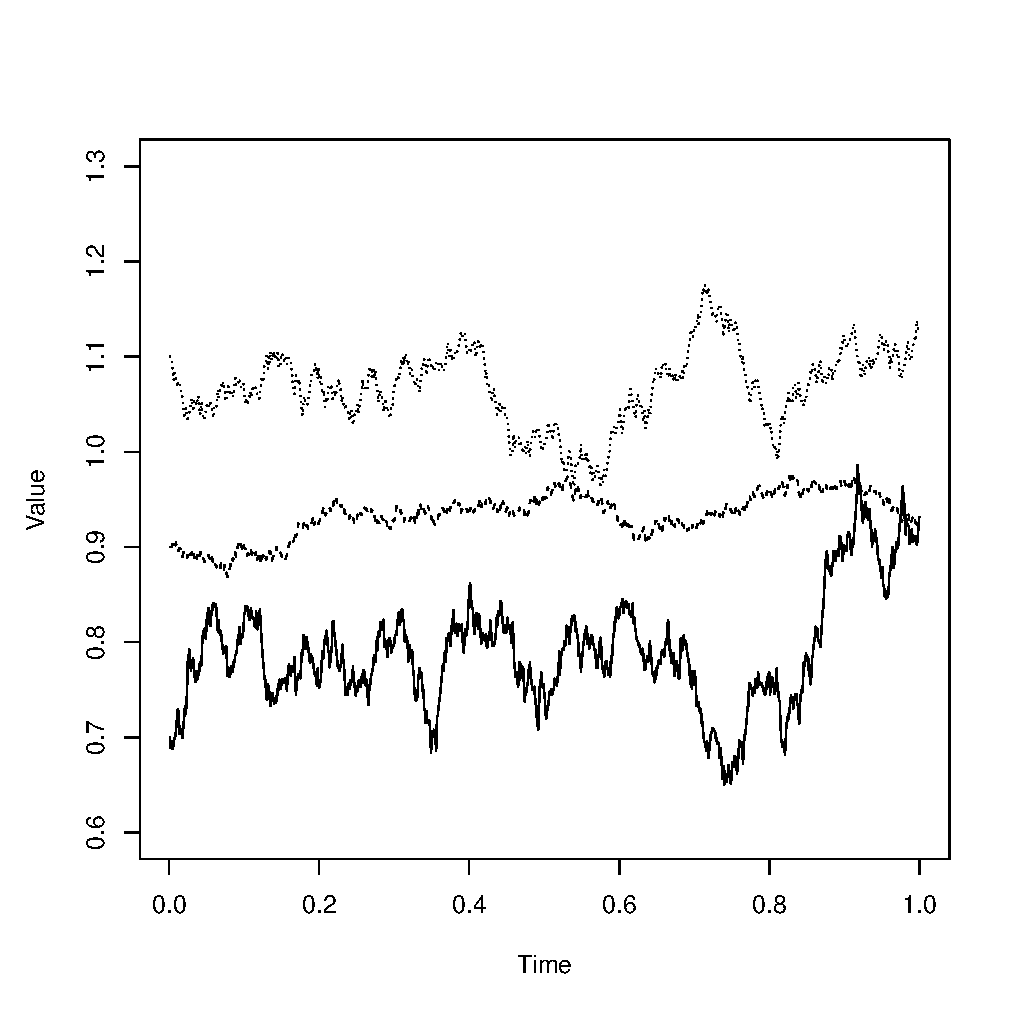
\includegraphics[width=1\textwidth]{StahlPaper2Z}
\caption{ \label{fig1}}
\end{minipage}\hfill
\begin{minipage}[t]{.48\textwidth}
\centering
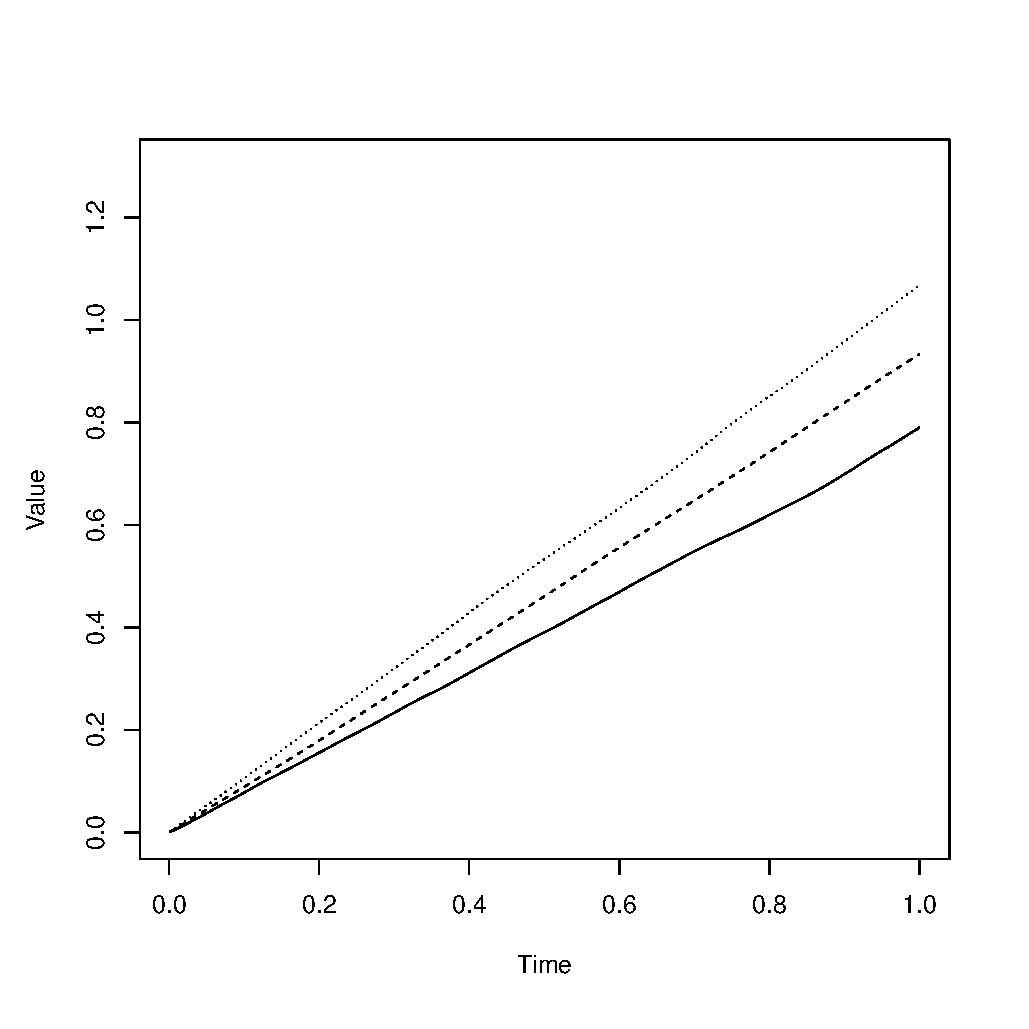
\includegraphics[width=1\textwidth]{StahlPaper2Y}
\caption{ \label{fig2}}
\end{minipage}\hfill
\end{framed}
\end{figure}


\begin{figure}[htb]
\begin{framed}
Sample paths of the probability of default\newline
\begin{minipage}[t]{.48\textwidth}
\centering
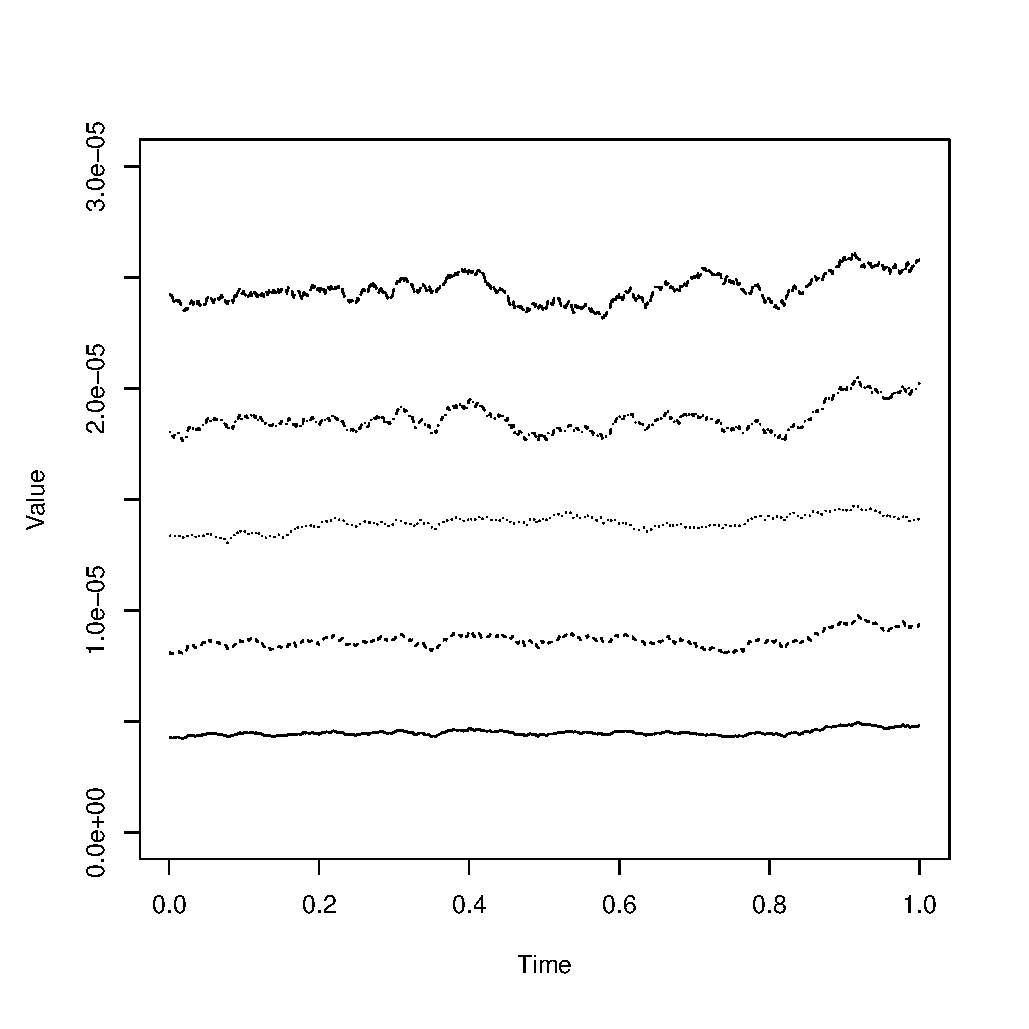
\includegraphics[width=1\textwidth]{StahlPaper2P}
\caption{Instantaneous probability of default \label{fig3}}
\end{minipage}\hfill
\begin{minipage}[t]{.48\textwidth}
\centering
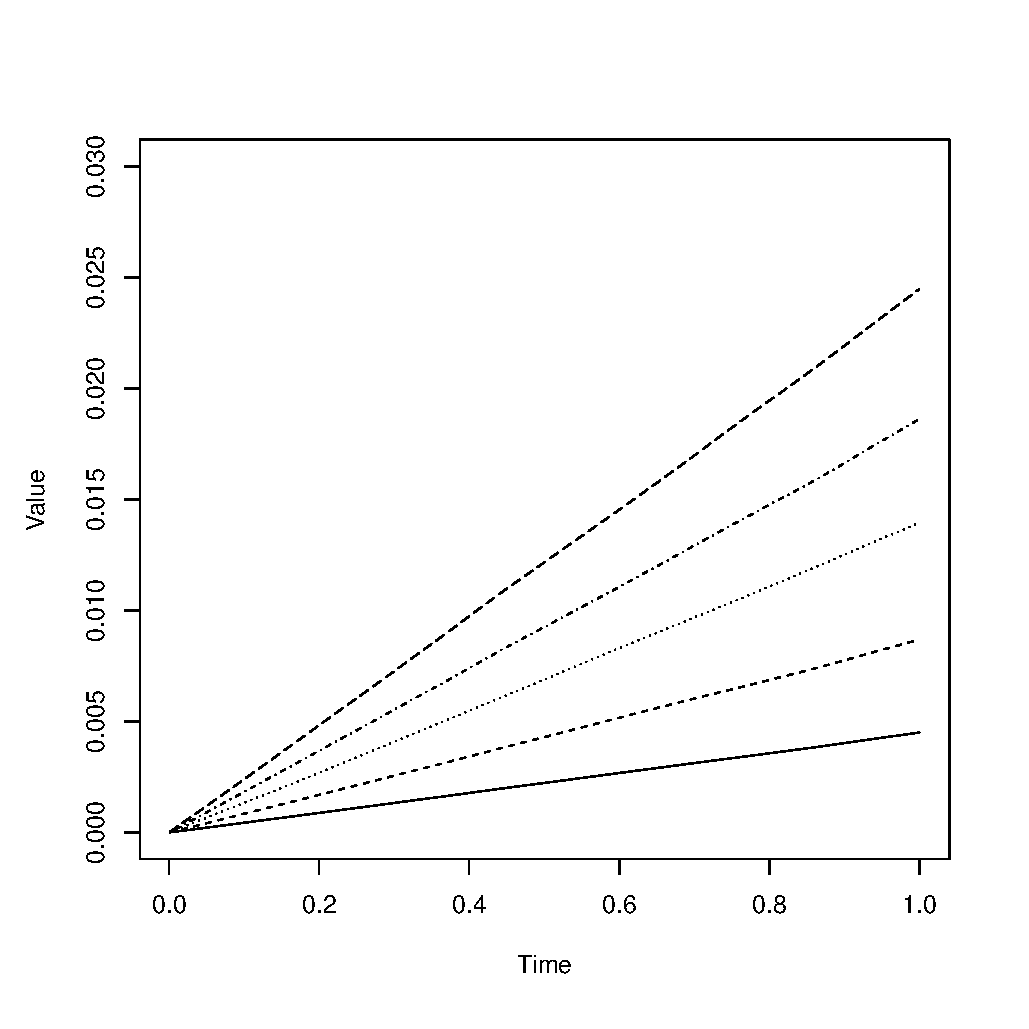
\includegraphics[width=1\textwidth]{StahlPaper2PY}
\caption{Cumulative probability of default \label{fig4}}
\end{minipage}\hfill
\end{framed}
\end{figure}

%\begin{equation}
%d\left[\begin{array}{l} L_1 \\ L_2 \\L_3 \end{array}\right]=
%\left[ \begin{array}{lll} .3 & 0& 0 \\ 0 & .2 & 0 \\ 0 & 0 & .1 \end{array} \right]\left(\left[\begin{array}{c} 1 \\1\\1 \end{array} \right] - \left[\begin{array}{l} L_1 \\ L_2 \\L_3 %\end{array}\right] \right) dt + 
%\left[\begin{array}{ccc} .2 & 0 & 0 \\ .02 & .09797959 & 0 \\ -.09 & .07960842 & .2748863 \end{array}\right]\left[\begin{array}{c} dW_t ^1 \\ dW_t ^2 \\ dW_t ^3\end{array} %\right]
%\end{equation}



\subsection{Total and Marginal Risk}

 For the sake of this example and without loss of generality, it will be assumed that the risk of the portfolio is adequately represented by \(\mathbb{E}[X_T^\lambda]+\sqrt{\mathbb{V}(X_T^\lambda)}\).  The following table summarizes the results.

\begin{table}[H]
\centering
\begin{tabular}{ccccccc}
&\(X_T^1\) & \(X_T^2\)& \(X_T^3\)& \(X_T^4\)& \(X_T^5\)  & Total\\
\hline
p& .005 & .01& .015& .02& .025 & \\
l & 987 &2104 & 1264 & 576 &377 &\\
r & .13 & .15 & .18 & .14 & .78  &\\
\(\rho_j\left(X_T^\lambda\right)\) & 27.62&159.80&103.83&36.08&42.38&369.70 \\
\(\rho_j\left(X_T ^ {\lambda^*}\right)\) & 23.03&170.37&110.02&39.19&27.09&369.70 \\
\(\rho_j(X_T)\) & 20.01&153.34&96.89&32.88&22.01&325.13 \\

\end{tabular}
\end{table}
\(X_T ^ {\lambda^*} \) represents the risk contributions without charging liquidity risk at the loan level: that is, equation (\ref{liquidRiskC}) is used (with \(\lambda_0=\lambda\)) instead of equation (\ref{liquidityRiskContributions}).  \(X_T ^ \lambda\) is superior at charging risk to the loans that truly add more to the riskiness of the portfolio.  The risk of \(X_T ^ 5\) is sharply increased over \(\rho_j (X_T)\) due to its relatively high \(r\), while the risk of \(X_T ^ 2\) barely increases.

\section{Conclusion}

\subsection{Applications}
\subsubsection{Granular Pricing of Risk}
There are three primary risks in the credit origination and servicing process: credit, liquidity, and interest rate risk.  This paper addresses credit and liquidity risk and presents a framework in which these two risks can be charged at the loan level.  Most banks hold liquidity risk capital at the top of the house and do not charge it to each loan (Grant 2011). While certainly there should be some liquidity capital held at the top of the house, there are significant liquidity idiosyncrasies within a loan portfolio.  Charging liquidity risk solely to the entire portfolio is akin to using a single probability of default for an entire portfolio: it is too broad to adequately capture the dynamics of risk within the portfolio.  It is unlikely that the pricing or origination decision of individual loans is optimal.  The methodology within this paper allows banks to optimally originate and price loans.

\subsubsection{Basel Compliance}

Basel III's guidance on the liquidity coverage ratio lists several fundamental characteristics of a``high quality liquid asset'' (HQLA) which is the numerator of a part of the liquidity coverage ratio (Basel 2013).  Among these characteristics are:

\begin{enumerate}
\item \textbf{Low risk}: assets that are less risky tend to have higher liquidity.
\item \textbf{Ease and certainty of valuation}: an asset's liquidity increases if market participants are more likely to agree on its valuation.  Assets with more standardized, homogeneous and simple structures tend to be more fungible, promoting liquidity.  The pricing formula of a high-quality liquid asset must be easy to calculate and not depend on strong assumptions.
\item \textbf{Low correlation with risk assets}: the stock of HQLA should not be subject to wrong-way (highly correlated) risk.
\end{enumerate}
The model in this paper addresses each of these characteristics.  
\begin{enumerate}
\item The liquidity risk concentration of each loan is increasing in \(p\) and \(l\), thus charging more liquidity capital to riskier loans. 
\item Loans with easier valuation (such as pledgable loans to the FHLB) will have less liquidity capital due to a lower \(r\).  
\item The liquidity capital charge is increasing in \(\sigma^2 (w, d)\)  which is the primary drivers of correlation between loans (see the appendices of Stahl (2015)).
\end{enumerate}

\subsubsection{Connection with Market Risk}
The third major risk in the loan origination and servicing process, interest rate risk, is typically hedged by swaps.  These swaps are part of a bank's trading book and are subject to the Market Risk Rule (Risk-Based Capital Guidelines 2012).  This rule requires certain amounts of capital to be held for market risk.  While most interest rate risk is hedged and capital charged via the Market Risk Rule, there remains additional interest rate risk for each loan.  As interest rates increase, floating rate loans will have increasing probabilities of default.  Even fixed rate loans' obligors may have cash flow sensitivity to interest rates that affect their default behavior.  This additional interest rate risk can be captured with the model presented in this paper by using interest rates as one of the factors effecting the probability of default.  In this way total interest rate risk can be decomposed into ``pure'' interest rate risk (cash flow risk to the bank hedged by swaps and with capital held as required by the Market Risk Rule) and credit interest rate risk (which is charged to the loan level).   Using interest rates as an input into the credit model may also lead to insite into the impact of correlations between market and credit risk.

\subsection{Further research}
The ``Holy Grail'' of economic capital models parsimoniously captures all major risk to the bank.  One method to accomplish this is by combining seperate models in an economically and mathematically meaningful manner.  The credit model presented in this paper can be quite easily integrated into other models.  For example, operational risk models frequently use characteristic functions (Temnov and Warnung 2008).  If some of the drivers that effect credit economic capital also effect operational risk then the joint distribution (including correlation) can be computed by multiplying the credit characteristic function and the operational characteristic function and numerically inverting to recover the density.  









\newpage

\begin{thebibliography}{9}
%\bibitem{creditriskplus}
%Credit Suisse. Creditrisk+: A credit risk management framework. Technical
%report, Credit Suisse First Boston, 2001.

\bibitem{artzner1999}
P. Artnzer, F. Delbaen, J. Eber, and D.Heath.  Coherent Measures of Risk.  \textit{Mathematical Finance},  1999.


\bibitem{baseliii}
Basel Committee on Banking Supervision. Basel III: The Liquidity Coverage Ratio and liquidity risk monitoring tools. Technical
report, Bank for International Settlements, 2013.

\bibitem{duffie2000}
D. Duffie,  J. Pan, K.  Singleton. Transform analysis and asset pricing for affine jump diffusions.
\textit{Econometrica}, 2000.

%\bibitem{fang2008}
%F. Fang and C.W. Oosterlee. A novel pricing method for european options
%based on fourier-cosine series expansions. \textit{SIAM Journal on Scientific Computing}, 2008.

\bibitem{Filipovic2001}
D. Filipovic. A general characterization of one factor affine term structure models. \textit{Finance and Stochastics}, 2001.


\bibitem{baselFSI}
J. Grant. Liquidity Transfer Pricing: a Guide to Better Practice.  \textit{Financial Stability Institute},  Bank for International Settlements, 2011.

\bibitem{Kalkbrener2005}
M. Kalkbrener. An axiomatic approach to capital allocation. \textit{Mathematical Finance}, 2005.

\bibitem{patrick1999}
G. Patrik, S. Bernegger, and M. Ruegg. The use of risk adjusted capital to support business decision
making. \textit{Casualty Actuarial Society Forum}, 1999.

\bibitem{marketRiskRule2012}
Risk-Based Capital Guidelines: Market Risk. 77 Fed. Reg. 53060, Aug. 30, 2012.

\bibitem{Stahl2015}
D. Stahl. Loss Distributions: Computational Efficiency in an Extended Framework. \textit{Journal of Credit Risk}, 2015.

\bibitem{tasche2007}
D. Tasche and C. Acerbi. Euler allocation: Theory and practice. \textit{Zentrum
Marhematic (SCA)}, 2007.

\bibitem{temnov2008}
G. Temnov and R. Warnung. A comparison of loss aggregation methods for operational risk. \textit{Journal of Operational Risk}, 2008 


\end{thebibliography}

\newpage
\appendix
%\section{Appendix} \label{appendix}

\section{Moments of \(Y_T\)} \label{mY}

\subsection{Expectation of \(z^T Y_T\)}
From equation (\ref{solutionL}) and using the fact that Ito integrals are martingales, 

\begin{equation}
\mathbb{E}[z^T L_T]=z^T \left(\mathbf{1}+e^{-AT}(L_0-\mathbf{1})\right)
\end{equation}
Integrating and using the fact that \(e^A\) is applied component-wise when \(A\) is diagonal,

\begin{equation}
\mathbb{E}[z^T Y_T]=\sum_{i=1} ^ m z_i T+\frac{z_i}{A_{i,i}}\left(1-e^{-{A}_{i, i}T}\right)(L_0^ i-1)\end{equation}

\subsection{Variance of \(z^T Y_T\)}
To find the variance of \(z^T Y_T\) I introduce the following lemma:

\begin{lemma} \label{lemma1}
Let \(I_t\) be a bounded Ito integral  and \(C_t\) be a Riemann integrable function.  Then 
\begin{equation} \label{fubini} \int_ 0^ T  C_t I_t dt=  \int_ 0^ T \left(\int_0 ^ T C_t  dt-\left(\int_0 ^ t C_s ds\right)\right) dI_t
\end{equation}

\end{lemma}

\begin{proof}
By Ito's Lemma,
\begin{equation}
d\left(\int_0 ^ T C_t dt\right) I_T= C_t I_t dt +\left(\int_0 ^ t C_s ds\right) dI_t
\end{equation}
Rearranging and integrating yields equation (\ref{fubini}).
\end{proof}

The only part of equation (\ref{solutionL}) that contributes the variance is the Ito integral.  Hence the problem of finding the variance reduces to 
\begin{equation}
\mathbb{V}(z^T Y_T)=\mathbb{V}\left(z^T \int_0 ^ T e^{-At} \int_ 0 ^ t e^{As} \Sigma dW_s dt \right)
\end{equation}

Letting \(C_t=e^{-At}\) and \(I_t=\int_ 0 ^ t e^{As} \Sigma dW_s \) and using lemma \ref{lemma1},

\begin{equation}
=\mathbb{V}\left(z^T  \int_ 0 ^ T \frac{1}{A}\left( e^{-At} -e^{-AT} \right) e^{At}\Sigma dW_t  \right)
\end{equation}
Where \(\frac{1}{A}\) is defined as component-wise division.
\begin{equation}
=\mathbb{V}\left(z^T  \int_ 0 ^ T \frac{1}{A}\left( \mathbf{I}-e^{-A(T-t)} \right)\Sigma dW_t  \right)
\end{equation}
Where  \(\mathbf{I}\) is the identity matrix.
\begin{equation}
=\int_ 0 ^ T z^T M_t \Sigma \Sigma ^T M_t^T z dt  
\end{equation}
Where \(M_t=\frac{1}{A}\left( \mathbf{I}-e^{-A(T-t)} \right)\).

\begin{equation}
=\int_0 ^ T \sum_{i=1} ^ m \sum_{j=1} ^ m z_i z_j \sigma_i \sigma_j \rho_{i,j} \frac{1}{A_{i,i}}\left(1-e^{-{A}_{i, i}(T-t)}\right)\frac{1}{A_{j,j}}\left(1-e^{-{A}_{j, j}(T-t)}\right) dt\end{equation}

Integrating yields equation (\ref{varianceY}).
\section{Moments of \(X_T\) and \(X_T ^ \lambda\)} \label{mX}

\subsection{Expectation of \(X_T\)}

\begin{equation}
\mathbb{E}[X_T]=\frac{\partial \phi_{X_T}}{\partial u} \big|_{u=0}
\end{equation}

\begin{equation}
 =\frac{\partial e^{\mu(z)+\frac{\sigma^2(z)}{2} }}{\partial u} \bigg|_{u=0}\end{equation}
 
 \begin{equation}
 = e^{\mu(z)+\frac{\sigma^2(z)}{2} } \left(\mu(z')+\frac{1}{2} \sigma^2 (z', \mathbf{1})\right) \bigg|_{u=0}\end{equation}
 
 \begin{equation}
 =\mu(d)
 \end{equation}
 Where \(d=z'=\frac{1}{i}\sum_j p_j \phi_j'(0) w_{j, k} \)
 
 \subsection{Variance of \(X_T\)}
 
\begin{equation}
\mathbb{V}(X_T)=\frac{\partial^2 \phi_{X_T}}{\partial u^2} \big|_{u=0}
\end{equation}

\begin{equation}
 =\frac{\partial ^2 e^{\mu(z)+\frac{\sigma^2(z)}{2} }}{\partial u^2} \bigg|_{u=0}\end{equation}
 
 \begin{equation}
 = e^{\mu(z)+\frac{\sigma^2(z)}{2} } \left(\mu(z'')+ \sigma^2 (z') \right) \bigg|_{u=0}\end{equation}
 
 \begin{equation}
 =\mu(d^2)+\sigma^2 (d)
 \end{equation}
 Where \(d^2=z''=-\sum_j p_j \phi_j''(0) w_{j, k} \)
 
 \subsection{Expectation of \(X_T ^ \lambda \)}


\begin{align} \mathbb{E}[X_T ^ \lambda]&=\frac{\partial \phi_{X_T}\left(u-iq(e^{u\lambda i}-1)\right) }{i\partial u} \bigg|_{u=0}\\
&=\frac{1}{i} \phi_{X_T}'\left(u-iq(e^{u\lambda i}-1)\right) \left(1+q\lambda e^{u\lambda i}\right) \big|_{u=0} \\
&=\frac{ \phi_{X_T}i ' (0)}{i}(1+q \lambda) = \mathbb{E}[X_T] (1+q \lambda)\end{align}

 
  \subsection{Variance of \(X_T ^ \lambda \)}

\begin{align}\mathbb{E}\left[{X_T^\lambda} ^2 \right]&=-\frac{\partial^2  }{\partial u^2} \phi_{X_T}\left(u-iq(e^{u\lambda i}-1)\right)\bigg|_{u=0}\\
&=-\phi_{X_T}i''\left(u-iq(e^{u\lambda i}-1)\right) \left(1+q  \lambda e^{u\lambda i} \right)^2 \big|_{u=0}\nonumber\\&+\frac{1}{i^2}\phi_{X_T}'\left(u+\frac{q(e^{u\lambda i}-1)}{i}\right)q i \lambda^2  e^{u\lambda i}   \big|_{u=0}  \\
&=-\phi_{X_T} '' (0)(1+q \lambda)^2+i\phi_{X_T}'(0)  q \lambda^2\\
&=\left(\mathbb{V}(X_T)+\mathbb{E}[X_T]^2 \right)(1+q\lambda)^2+\mathbb{E}[X_T]q\lambda^2 \end{align}
\begin{align} \mathbb{V}(X_T ^ \lambda)&=\left(\mathbb{V}[X_T]+\mathbb{E}[X_T]^2 \right)(1+q\lambda)^2+\mathbb{E}[X_T]q\lambda^2-\mathbb{E}[X_T]^2(1+q\lambda)^2\\
&=\mathbb{V}(X_T)(1+q\lambda)^2+\mathbb{E}[X_T]q\lambda^2\end{align}
%\[=\left(\mu_Y T \sigma^2 - \sigma^2 T^2 + \sigma^2  \frac{T^3}{3}+\sigma^2 \frac{Z_0-1}{\alpha} e^{-\alpha T} T^2\right)(1+q \lambda)^2+ \mathbb{E}[X] q \lambda ^2\]

\section{Risk Contributions} \label{rc}
The risk contribution for a standard deviation based risk measure is 
\begin{equation}
\rho_{X_T^j}=\mu_j+c\frac{\mathrm{cov}(X_T ^ j,\,X_T)}{\sigma_{X_T}}
\end{equation}

From equation (\ref{meX}), 
\begin{equation}
\mu_j=\mu\left(\frac{1}{i} p_j \phi_j'(0) w_{j, k}\right)=\frac{1}{i} p_j \phi_j'(0) \mu\left( w_{j}\right)
\end{equation}
Where \(\mu(\cdot)\) is defined as in equation (\ref{meY}).  
\\
\\
By Euler's theorem (\ref{euler}) the sum of the contributions will equal to the total risk.  The only way to decompose equation (\ref{mvX}) such that the sum of the component parts equals the whole is by taking the ``difference'' of the equation such that only ``\(j\)'' components effect the \(j\)'th contribution.  Straightforward but tedious computation yields equation (\ref{rcX}).  A similar argument leads to equation (\ref{liquidRiskC}).  The argument does not work for \(X_T ^ \lambda\) since there are multiple ways to take the ``difference'': \(\lambda\mathbb{E}[X_T]\) can be split into \(r_j b_j \mathbb{E}[X_T]\) or into \(-\frac{1}{i}\lambda p_j \phi_j '(0) \mu(w_j)\).  Hence the additional criteria outlined in (\ref{criteria}) are necessary.


%The key takeaway is that \emph{no  optimization must be done}.  The economic capital must be pushed down to the individual loan officers and by tying this capital to their compensation they will automatically choose an optimal allocation of loans.  

%\section{Expected Value [no liquidity]}
%Letting \(d\) be the vector \(d=\sum_j p_j l_j w_{j, k}\), 
%\[\mathbb{E}[X]=\mu(d) \]

%\section{Variance[No liquidity]}
%Letting \(d ^2\) be the vector \(d^2=\sum_j p_j l_j^2 w_{j, k}\),
%\[\mathbb{V}(X)=\mu(d ^2)+\sigma^2(d)\]



\end{document}
